
\subsection{GUI}

V rámci kapitoly \ref{popis-gui} jsme specifikovali požadavky, které máme na uživatelské
rozhraní.
V této kapitole se detailněji podíváme na implementaci celého GUI.

%\begin{figure}[tbh!]\centering
%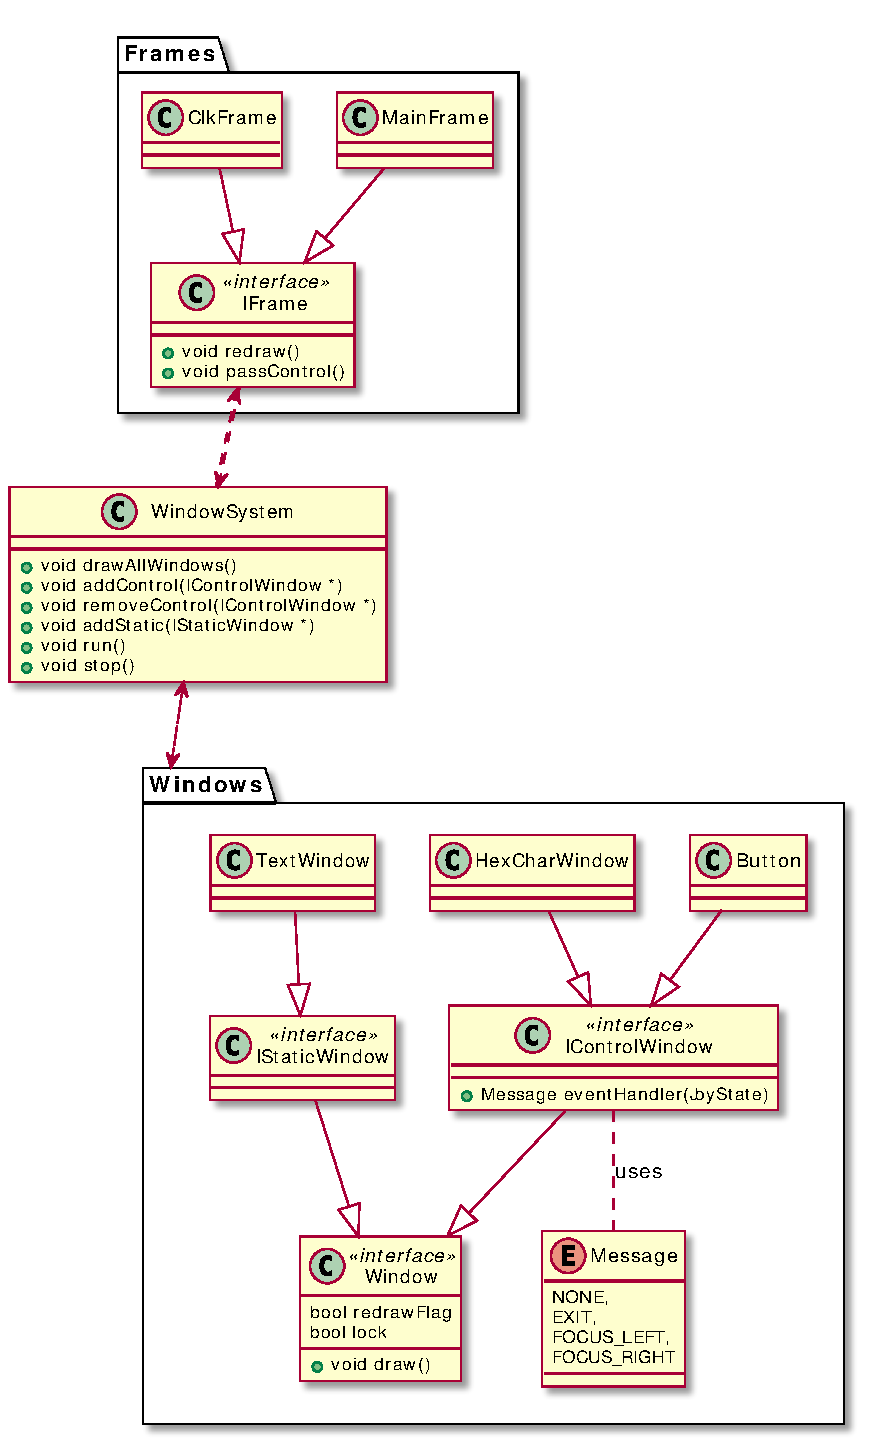
\includegraphics[scale=0.75]{../diagrams/stm_gui.pdf}
%\caption{Hierarchie základních tříd v GUI}
%\label{fig:stm-gui}
%\end{figure}

Obrázek (TODO: odkaz) zobrazuje hierarchii základních tříd a vztahy mezi nimi.
Pro jednoduchost zobrazuje pouze pár konkrétních tříd jako příklad: \texttt{TextWindow} jako statické
okno, které pouze zobrazuje text a \texttt{HexCharWindow} jako kontrolní okno, které je součástí
\texttt{KeyFrame} a zobrazuje právě jeden hexadecimální znak, jehož hodnotu může uživatel
zvětšovat či změnšovat.
Celé GUI je tvořeno dvěma základními druhy objektů - \emph{windows} a \emph{frames}.
Každý frame reprezentuje jednu obrazovku tj. co všechno je v daný moment zobrazeno na displeji.
Windows jsou velice jednoduchá okna - typicky zobrazující pouze neohraničený text resp. číselnou
hodnotu.
Frame obsahuje několik oken a definuje, kde přesně mají tato okna být zobrazena a jakého typu
mají být.
Každý frame má svůj \texttt{WindowSystem}, přes který může sám do sebe vkládat okna.
Kromě toho, že \texttt{WindowSystem} zpracovává vstup, na základě kterého přepíná mezi jednotlivými okny,
funguje také jako prostředník mezi frame a jeho okny.

% Windows
\subsubsection{Windows}
% static and control windows
Window může být buď \emph{statické} (dědí od třídy \texttt{IStaticWindow}), nebo \emph{kontrolní}
(dědí od třídy \texttt{IControlWindow}).
Statické okno slouží pouze pro zobrazování libovolného textu, kontrolní okno může uživatel \uv{nakliknout}
a změnit jeho hodnotu.
Jediný uživatelský vstup je joystick a řekněme, že jeho zmáčknutím doprava nebo doleva se uživatel
přesune mezi jednotlivými okny, a zmáčknutím nahoru nebo dolů může uživatel měnit hodnotu
v právě nakliknutém okně.
Přímé stisknutí joysticku má vliv pouze na okna typu \texttt{Button}, která typicky slouží buď jako
potvrzení všech zadaných hodnot v rámci jedné obrazovky, nebo jako \uv{exit} tlačítko.
Možnost nakliknutí a změny nějaké hodnoty kontrolního okna se do objektového návrhu promítá tak,
že \texttt{IControlWindow} má čistě virtuální metodu \texttt{Message eventHandler(JoyState joyState)}.
Zjednodušeně řečeno každé okno pomocí přetížení této metody specifikuje svoji reakci na vstup,
kde tato reakce může být buď čistě interního charakteru tj. změna hodnot daného okna, nebo může
vrátit jednu z hodnot \texttt{Message::FOCUS\_LEFT} nebo \texttt{Message::FOCUS\_RIGHT}, čímž
říká, že nakliknuté má být kontrolní okno, které je vlevo nebo vpravo od tohoto okna, případně
může vrátit \texttt{Message::EXIT}, čímž říká že má být aktuální frame vypnut.

% WindowSystem
\subsubsection{WindowSystem}
\texttt{WindowSystem} je v podstatě kontejner pro všechna okna v rámci jednoho frame a ještě se stará
o výše zmíněnou logiku.
Frame Při inicializaci pouze přidává kontrolní a statická okna do \texttt{WindowSystem}.
Za běhu potom \texttt{WindowSystem} podle vstupu buď přepíná mezi kontrolními okny, nebo přímo vypne
aktuální frame.

% zpracování vstupu je v interrupt handleru kdežto vykreslování v mainloop
Zde je důležité si uvědomit, že zpracování vstupu probíhá v \emph{user input task}, což je interrupt
handler jednoho z timeru, který tento interrupt spouští jednou za 100 ms.
Z pohledu kódu je tedy zpracování vstupu a všechno s tím spojené asynchronní.
Protože zpracování vstupu běží v jiném kontextu než vykreslování, je potřeba rozlišovat metody podle
toho ve kterém kontextu jsou volány.
Označme metody volané v kontextu zpracování vstupu jako \emph{callback} metody a definujme pro
ně strukturu, kterou rozebereme v následujícím odstavci.

%%%%% Callback metody %%%%%%
\paragraph{Callback metody}
Občas v rámci jednoho frame chceme reagovat na stisknutí některého z čudlíků.
Například při stisku \uv{Exit} v \texttt{SetIntervalFrame} bychom chtěli ukončit celý frame a uložit
uživatelem zadané hodnoty.
Zavedeme několik rozhraní se dvěmi čistě virtuálními metodami: \texttt{callback} a \texttt{register}.
\footnote{Přesný název konkrétních metod se liší, ale callback nebo register je jejich součástí}
\texttt{register} metoda by měla objekt, který chce dostávat callbacky zaregistrovat k jejich zdroji.
\texttt{callback} metoda potom implementuje reakci na konkrétní callback.
Všechny tyto rozhraní dědí od \texttt{ICallbackReceiver}.

Myšlenka je taková, že když chceme, aby objekt A dostával určité callbacky od objektu B,
musíme nejprve objekt A u objektu B registrovat jako \uv{callback receiver} a potom definovat
metodu která na tento callback bude reagovat.

Místo toho, abychom vyjmenovali všechny možné typy callbacků a jejich parametry, zpřesníme
strukturu callback metod na příkladě.

%\begin{figure}[tbh!]\centering
%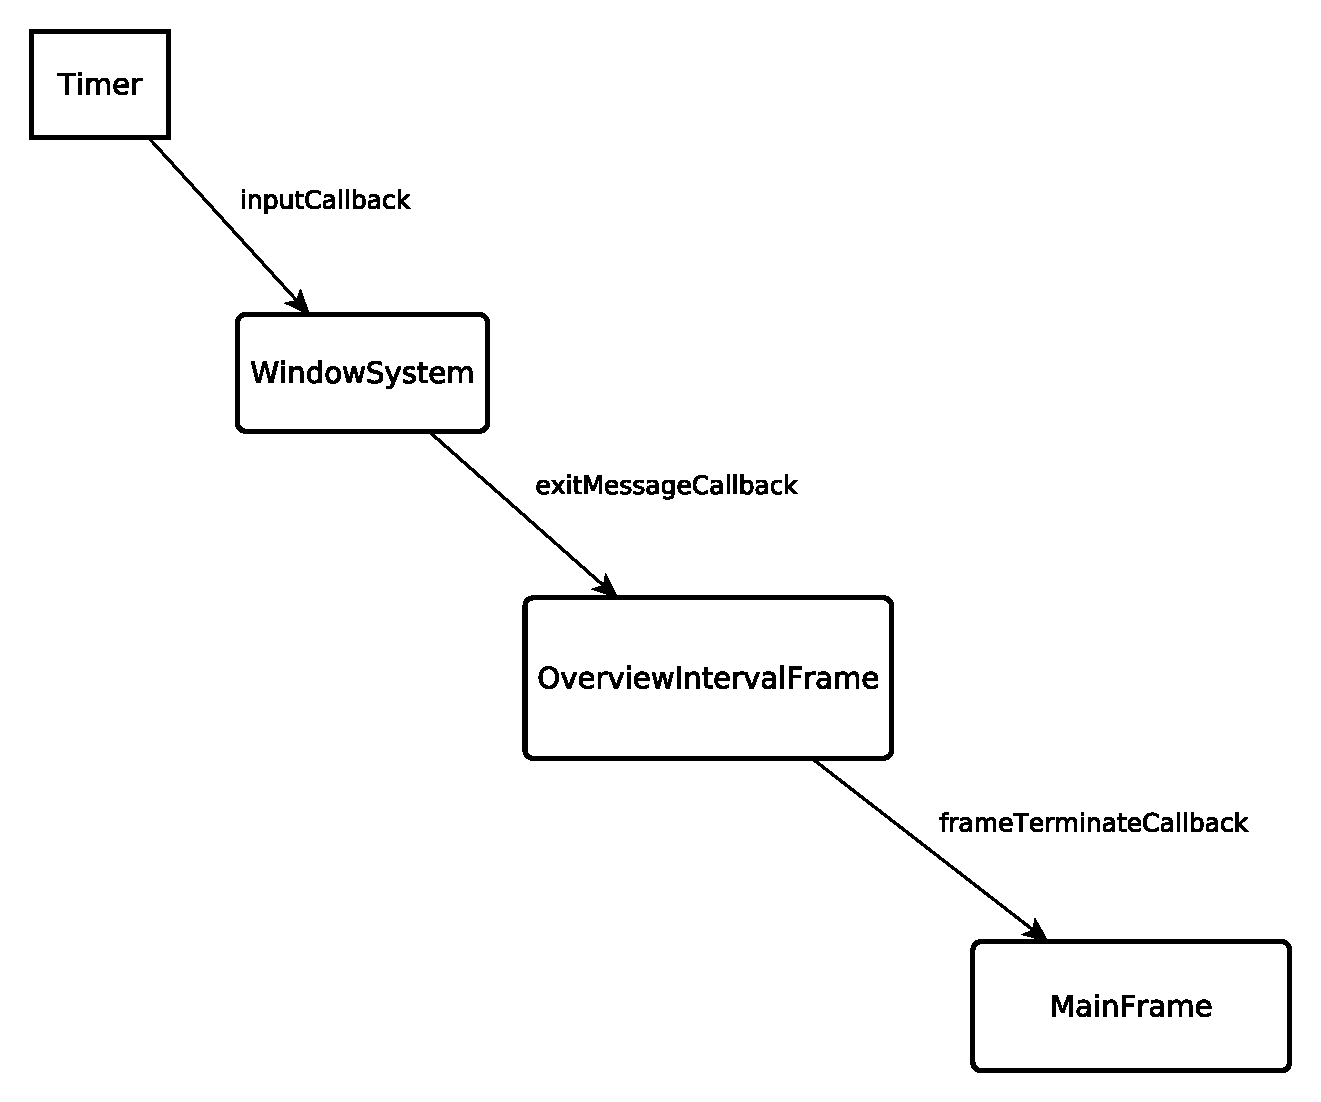
\includegraphics[scale=0.6]{../diagrams/stm_callback_metody.pdf}
%\caption{Příklad hierarchie volání callback metod}
%\label{fig:stm-callback-metody}
%\end{figure}

Diagram (TODO: odkaz) ilustruje situaci, kdy je uživatel v \texttt{OverviewIntervalFrame}, stiskne
tlačítko \uv{exit} a dostane se zpět do \texttt{MainFrame}.
Proces na diagramu je následující:
\begin{enumerate}
  \item Vygenerování interruptu timerem.
  \item Zavolání metody \texttt{IO::task}, ve které dojde k vytvoření callback objektu s parametrem.
  \item Zavolání metody \texttt{WindowSystem::inputCallback}, která tento callback předá aktuálně
    nakliknutému oknu (v tomto případě je to \texttt{exitButton}), které vrátí \texttt{Message::EXIT}
    ze svého \texttt{eventHandler}.
  \item Zavolání metody \texttt{OverviewIntervalFrame::exitMessageCallback}
  \item Zavolání metody \texttt{MainFrame::frameTerminateCallback}, ve které MainFrame určí který
    frame skončil a nastaví sám sebe jako aktuální frame.
\end{enumerate}
%%%%%% konec callback metod %%%%%%%

% přístup k oknům z interrupt handleru/mainloopu --> nutnost zamykání
Celý tento \uv{framework} je navržen s ohledem na co nejsnazší specifikaci vzhledu i chování nově přidávaného
framu, ale také s ohledem na to, že čtení vstupu probíhá v kontextu interrupt handleru, kdežto vykreslování
oken probíhá v \emph{mainloop}.
Mohlo by se tedy stát, že vykreslování okna bude přerušeno, v interrupt handleru se změní jeho hodnoty,
a vykreslování se opět obnoví - toto může vést k tomu, že okno vykreslí špatné hodnoty.
Každé okno má tedy zámek, který je zamčen před voláním metody \texttt{draw} nebo metody \texttt{eventHandler}.
O toto zamykání se nemusí starat programátor při definování nového okna, děje se totiž už na úrovni
třídy \texttt{Window}.

% okna se nepřekreslují, když to není nutné.
Pokud oknu změníme hodnotu a chceme, aby bylo v rámci \emph{GUI task} překresleno, musíme mu explicitně
nastavit \texttt{redrawFlag}.
Díky redrawFlag máme zajištěno i to, že nemusíme zbytečně překreslovat okna, která to nepotřebují.
Přeci jen je vykreslování na displej časově poměrně náročné.

